\definecolor{pem}{HTML}{ffc042}
\definecolor{steel}{HTML}{ffffff}
\definecolor{fluid}{HTML}{99c2f0}
\definecolor{rubber}{HTML}{d15700}

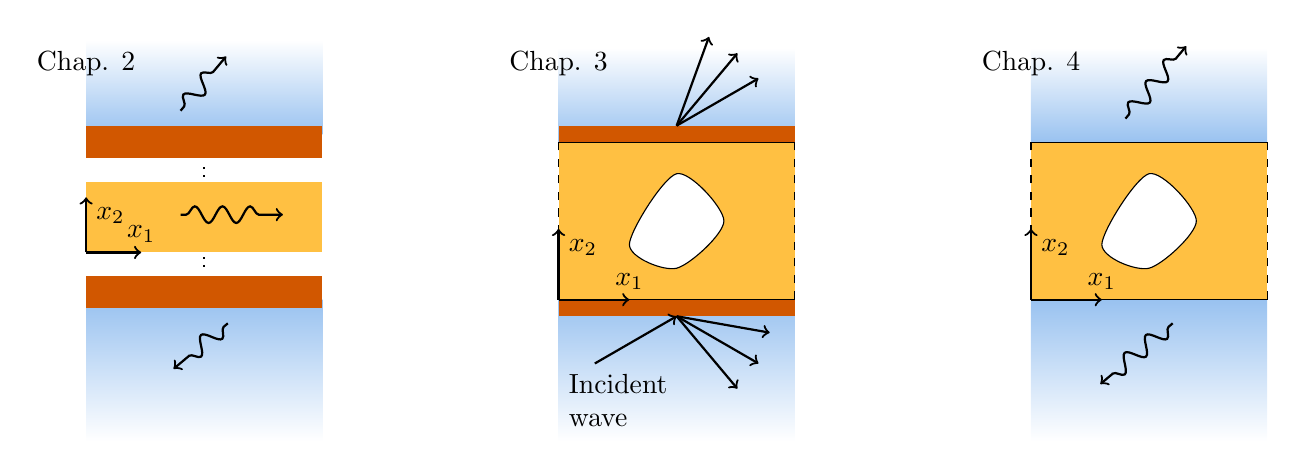
\begin{tikzpicture}
    \def\len{3}
    \def\height{1.5}
    \def\chapwidth{6cm}
     \def\pad{.3} 
    % CHAPTER 2
    \begin{scope}       
    \def\arrow{.7}
        \draw[top color = white, bottom color=fluid, draw=none] (0, \height+2*\pad) rectangle ++ (\len, 4*\pad);
        \draw[top color = fluid, bottom color = white,draw=none] (0, 0) rectangle ++ (\len, -6*\pad);
        \draw[fill=pem, draw=none] (0, 2*\pad) rectangle ++ (\len, \height-2*\pad);
        \draw[thick, dotted] (\len/2, \height+.2*\pad) -- ++ (0, .5*\pad);
        \draw[thick, dotted] (\len/2, 2*\pad-.2*\pad) -- ++ (0, -.5*\pad);
        \draw[fill=rubber, draw=none] (0, \height+\pad) rectangle ++ (\len, .4);
        \draw[fill=rubber, draw=none] (0, \pad) rectangle ++ (\len, -.4);
            \draw[thick,->] (0,2*\pad) -- ++ (\arrow, 0) node[above] {$x_1$};
    \draw[thick, ->] (0,2*\pad) -- ++ (0, \arrow) node[below right] {$x_2$};
    \draw[->,thick,decorate,decoration={snake,amplitude=3pt,pre length=2pt,post length=3pt}] (\len/2-\pad, \height+3*\pad) -- ++ (50:3*\pad) node[right] {};
    \draw[->,thick, decorate,decoration={snake,amplitude=3pt,pre length=2pt,post length=3pt}] (\len/2+\pad, -\pad) -- ++ (220:3*\pad) node[right] {};
        \draw[->,thick, decorate,decoration={snake,amplitude=3pt,pre length=2pt,post length=4pt}] (\len/2-\pad, \height-1.4*\pad) -- ++ (1.3, 0) node[right] {};
        \node at (0, 3) {Chap. 2};
    \end{scope}    
    % CHAPTER 3
    \begin{scope}[xshift=\chapwidth]   
    \def\cellen{\len} \def\height{2}\def\arrow{.9}\def\totalen{\cellen}
    \def\rubberthick{.7*\pad}
    \draw[top color = white, bottom color=fluid, draw=none] (0, \height) rectangle ++ (\totalen, 4*\pad);
    \draw[top color = fluid, bottom color = white,draw=none] (0, 0) rectangle ++ (\totalen, -6*\pad);
    \draw[fill=pem, draw=none] (0, 0) rectangle ++ (\totalen, \height);
    \draw[fill=rubber, draw=none] (0, \height) rectangle ++ (\totalen, \rubberthick);
    \draw[fill=rubber, draw=none] (0, 0) rectangle ++ (\totalen, -\rubberthick);

    \draw[black] (0, 0) -- ++ (\totalen, 0);
    \draw[black] (0, \height) -- ++ (\totalen, 0);
    \foreach \i in {0} {
            \draw[fill=white] plot[smooth cycle] coordinates {
            (\i*\cellen + \cellen/2, \height/2-2*\pad) 
            (\i*\cellen + \cellen/2 - 2*\pad, \height/2-\pad)
            % (\i*\cellen + \cellen/2-1.3*\pad, \height/2)
            (\i*\cellen + \cellen/2, \height/2+2*\pad)
            (\i*\cellen + \cellen/2 + 2*\pad, \height/2)
        };        
        \draw[dashed] (\i*\cellen, 0) -- ++ (0, \height);
        \draw[dashed] (\i*\cellen+\cellen, 0) -- ++ (0, \height);
        }
        
    \draw[thick,->] (0, 0) -- ++ (\arrow, 0) node[above] {$x_1$};
    \draw[thick, ->] (0, 0) -- ++ (0, \arrow) node[below right] {$x_2$};

    \draw[thick, ->] (\cellen/2, \height+\rubberthick) -- ++ (50:4*\pad) node[right] {};
    \draw[thick, ->] (\cellen/2, \height+\rubberthick) -- ++ (30:4*\pad) node[right] {};
    \draw[thick, ->] (\cellen/2, \height+\rubberthick) -- ++ (70:4*\pad) node[right] {};
    \draw[thick, <-] (\cellen/2, -\rubberthick) -- ++ (210:4*\pad)  node[below, xshift=12pt, text width=1.5cm] {Incident wave};
    \draw[thick, ->] (\cellen/2, -\rubberthick) -- ++ (-30:4*\pad) node[right] {};
    \draw[thick, ->] (\cellen/2, -\rubberthick) -- ++ (-50:4*\pad);
    \draw[thick, ->] (\cellen/2, -\rubberthick) -- ++ (-10:4*\pad);
    % \draw[dashed]    (\cellen/2, -\rubberthick) -- ++ (0, -4*\pad);

    \node at (0, 3) {Chap. 3};

\end{scope}  
%     % CHAPTER 4
    \begin{scope}[xshift=2*\chapwidth]   
\def\cellen{\len} \def\height{2}\def\arrow{.9}\def\totalen{\cellen}
    \def\rubberthick{.7*\pad}
    \draw[top color = white, bottom color=fluid, draw=none] (0, \height) rectangle ++ (\totalen, 4*\pad);
    \draw[top color = fluid, bottom color = white,draw=none] (0, 0) rectangle ++ (\totalen, -6*\pad);
    \draw[fill=pem, draw=none] (0, 0) rectangle ++ (\totalen, \height);

    \draw[black] (0, 0) -- ++ (\totalen, 0);
    \draw[black] (0, \height) -- ++ (\totalen, 0);
    \foreach \i in {0} {
            \draw[fill=white] plot[smooth cycle] coordinates {
            (\i*\cellen + \cellen/2, \height/2-2*\pad) 
            (\i*\cellen + \cellen/2 - 2*\pad, \height/2-\pad)
            % (\i*\cellen + \cellen/2-1.3*\pad, \height/2)
            (\i*\cellen + \cellen/2, \height/2+2*\pad)
            (\i*\cellen + \cellen/2 + 2*\pad, \height/2)
        };        
        \draw[dashed] (\i*\cellen, 0) -- ++ (0, \height);
        \draw[dashed] (\i*\cellen+\cellen, 0) -- ++ (0, \height);
        }
        
    \draw[thick,->] (0, 0) -- ++ (\arrow, 0) node[above] {$x_1$};
    \draw[thick, ->] (0, 0) -- ++ (0, \arrow) node[below right] {$x_2$};

    \draw[->,thick,decorate,decoration={snake,amplitude=3pt,pre length=2pt,post length=3pt}] (\cellen/2-\pad, \height+\pad) -- ++ (50:4*\pad) node[right] {};
    \draw[->,thick, decorate,decoration={snake,amplitude=3pt,pre length=2pt,post length=3pt}] (\cellen/2+\pad, -\pad) -- ++ (220:4*\pad) node[right] {};
    \node at (0, 3) {Chap. 4};
    \end{scope}  
\end{tikzpicture}